\begin{frame}{\texttt{pf} $+$ \texttt{sm2} $+$ feedback}

  \noindent\makebox[\linewidth][c]{%
  \begin{minipage}{\linewidth}
    \begin{minipage}{0.3\linewidth}
      \begin{figure}
        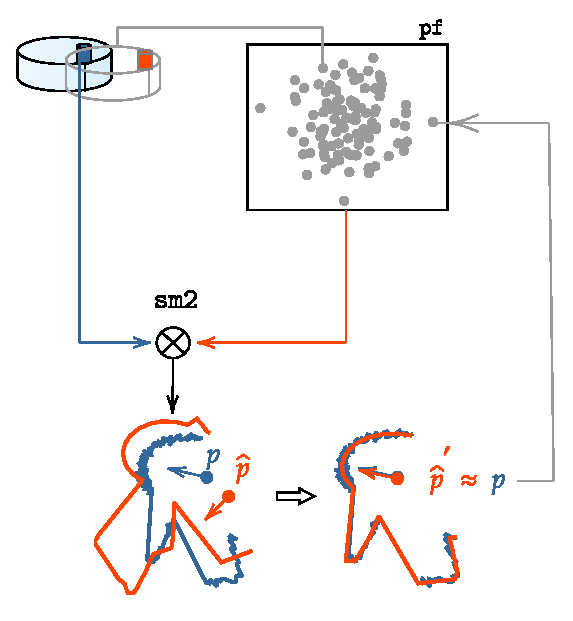
\includegraphics[width=120pt]{./figures/slides/ch4/smsm_pf_feedback.eps}
        \caption{\tiny  \texttt{sm2} προσαρμοσμένη στην έξοδο φίλτρου σωματιδίων (\texttt{pf}) και
                 ανάδραση της εξόδου της}
      \end{figure}
    \end{minipage}
    \hspace{1.2cm}
    \begin{minipage}{0.6\linewidth}
      \begin{figure}
        
\definecolor{r}{RGB}{255 69 0}
\definecolor{b}{RGB}{51 102 153}



\tikzset{every picture/.style={line width=0.75pt}} %set default line width to 0.75pt

\begin{tikzpicture}[x=0.75pt,y=0.75pt,yscale=-1,xscale=1]
%uncomment if require: \path (0,300); %set diagram left start at 0, and has height of 300

%Shape: Rectangle [id:dp6131376592433888]
\draw  [dash pattern={on 0.84pt off 2.51pt}] (322,78) -- (519.5,78) -- (519.5,157) -- (322,157) -- cycle ;
%Straight Lines [id:da45736430417167373]
\draw    (294.5,111) -- (325.5,111) ;
\draw [shift={(327.5,111)}, rotate = 180] [color={rgb, 255:red, 0; green, 0; blue, 0 }  ][line width=0.75]    (10.93,-3.29) .. controls (6.95,-1.4) and (3.31,-0.3) .. (0,0) .. controls (3.31,0.3) and (6.95,1.4) .. (10.93,3.29)   ;
%Straight Lines [id:da7019178260598848]
\draw   [color={rgb, 255:red, 51; green, 102; blue, 153 }  ] (293.5,172) -- (470.53,141.34) ;
\draw [shift={(472.5,141)}, rotate = 170.17] [color={rgb, 255:red, 51; green, 102; blue, 153 }  ][line width=0.75]    (10.93,-3.29) .. controls (6.95,-1.4) and (3.31,-0.3) .. (0,0) .. controls (3.31,0.3) and (6.95,1.4) .. (10.93,3.29)   ;
%Straight Lines [id:da9869567554869965]
\draw   [color={rgb, 255:red, 255; green, 69; blue, 0 }  ] (409.5,109) -- (470.56,123.51) ;
\draw [shift={(472.5,124)}, rotate = 194.04] [color={rgb, 255:red, 255; green, 69; blue, 0 }  ][line width=0.75]    (10.93,-3.29) .. controls (6.95,-1.4) and (3.31,-0.3) .. (0,0) .. controls (3.31,0.3) and (6.95,1.4) .. (10.93,3.29)   ;
%Straight Lines [id:da23755426444121874]
\draw    (397.5,37) -- (397.5,89) ;
\draw [shift={(397.5,91)}, rotate = 270] [color={rgb, 255:red, 0; green, 0; blue, 0 }  ][line width=0.75]    (10.93,-3.29) .. controls (6.95,-1.4) and (3.31,-0.3) .. (0,0) .. controls (3.31,0.3) and (6.95,1.4) .. (10.93,3.29)   ;
%Straight Lines [id:da07285087411586999]
\draw   [color={rgb, 255:red, 255; green, 69; blue, 0 }  ] (397.5,37) -- (487.97,112.72) ;
\draw [shift={(489.5,114)}, rotate = 219.93] [color={rgb, 255:red, 255; green, 69; blue, 0 }  ][line width=0.75]    (10.93,-3.29) .. controls (6.95,-1.4) and (3.31,-0.3) .. (0,0) .. controls (3.31,0.3) and (6.95,1.4) .. (10.93,3.29)   ;
%Straight Lines [id:da25729544560038]
\draw    (504.5,132) -- (543.5,132) ;
\draw [shift={(545.5,132)}, rotate = 180] [color={rgb, 255:red, 0; green, 0; blue, 0 }  ][line width=0.75]    (10.93,-3.29) .. controls (6.95,-1.4) and (3.31,-0.3) .. (0,0) .. controls (3.31,0.3) and (6.95,1.4) .. (10.93,3.29)   ;

% Text Node
\draw    (477,119) -- (505,119) -- (505,144) -- (477,144) -- cycle  ;
\draw (491,131.5) node   [align=left] {\texttt{sm}};
% Text Node
\draw (489,58) node [anchor=north west][inner sep=0.75pt]   [align=left] {\texttt{sm2}};
% Text Node
\draw (259,165) node [anchor=north west][inner sep=0.75pt]   [align=left] {$\textcolor{b}{\mathcal{S}(\bm{p})}$};
% Text Node
\draw (224,103) node [anchor=north west][inner sep=0.75pt]   [align=left] {Χάρτης $\bm{M}$};
% Text Node
\draw    (332.1,96) -- (409.1,96) -- (409.1,121) -- (332.1,121) -- cycle  ;
\draw (370.6,111) node   [align=left] {\texttt{scan\_map}};
% Text Node
\draw (393,16) node [anchor=north west][inner sep=0.75pt]   [align=left] {$\textcolor{r}{\hat{\bm{p}}}$};
% Text Node
\draw (422,95) node [anchor=north west][inner sep=0.75pt]   [align=left] {\footnotesize$\textcolor{r}{\mathcal{S}(\hat{\bm{p}})}$};
% Text Node
\draw (549,127) node [anchor=north west][inner sep=0.75pt]   [align=left] {$\textcolor{b}{\bm{p}}$};
\draw  [color={rgb, 255:red, 0; green, 255; blue, 0 }  ]  (556, 133) circle [x radius= 12.26, y radius= 12.26]   ;

\end{tikzpicture}

        \caption{\tiny  \texttt{sm2}: ευθυγράμμιση πραγματικής σάρωσης με εικονική σάρωση χάρτη}
      \end{figure}
    \end{minipage}

  \end{minipage}
  }

\note{\footnotesize
Αυτή η δεύτερη εκτίμηση είναι μία υπόθεση για την οποία το ίδιο το φίλτρο δεν
έχει γνώση, και συνεπώς θα ήταν ωφέλιμο, εάν η υπόθεση φέρει όντως μικρότερο
σφάλμα, να εισαχθεί στον πληθυσμό του, ώστε το σφάλμα του ίδιου το φίλτρου
να μειωθεί.}


\end{frame}
